\newcommand{\RM}[1]{\MakeUppercase{\romannumeral #1{}}}

\chapter{Tunneldiode\label{chapter:tunneldiode}}
\lhead{Tunneldiode}
\begin{refsection}
\chapterauthor{Stefan Hedinger}

\newpage
\section{Einleitung}
\rhead{Einleitung}
Die Tunneldiode ist ein nicht sehr h"aufig verwendetes, aktives und dynamisches Halbleiterelement. Die beiden Seiten des p-n-"Ubergangs sind stark dotiert. Durch den besonderen Aufbau und die starke Dotierung k"onnen Elektronen die Sperrschicht passieren bevor die Diode leitet.

Sie hat eine spezielle Kennlinie, welche im mittleren Bereich einen negativen Widerstand aufweist.

\begin{figure}[h]	%Bild Kennlinie der Tunneldiode
\centering
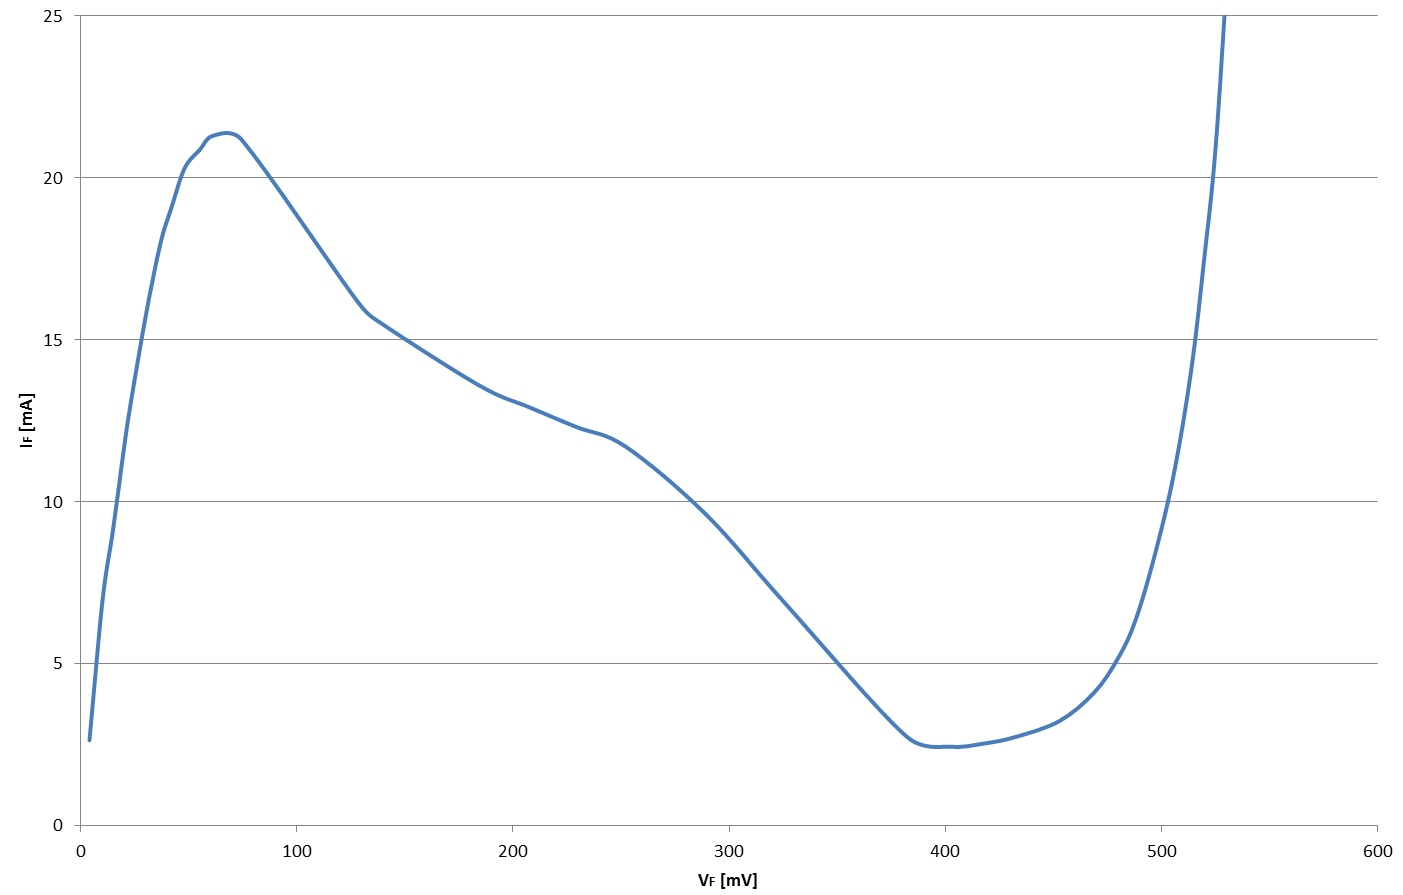
\includegraphics[width=0.7\textwidth]{tunneldiode/images/Tunneldiode.png}
\caption{Die spezielle Kennlinie der Tunneldiode
\label{skript:Tunneldiode}}
\end{figure}

\section{Tunneleffekt}
\rhead{Tunneleffekt}
Die Vorg"ange in der Tunneldiode werden mit dem Tunneleffekt beschrieben. Zum besseren Verst"andnis betrachten wir das Potential 
\[
V(x)=\begin{cases}
V_0& \qquad \text{wenn } x \in [-a,a]\\
0&   \qquad \text{sonst}
\end{cases}
\]
in den verschiedenen Bereichen.

Ein Teilchen kommt von links und m"ochte nach rechts. Die Energie vom einfallenden Teilchen ist $E$ und es gilt
\[
0 < E < V_0.
\]
In der Mitte ist aber eine Barriere, welche ein h"oheres Potential als das Teilchen selber aufweist. In der normalen Mechanik ist klar, dass dieses Teilchen nicht von links nach rechts kommt sondern an der Barriere bei -a reflektiert wird. In der Quantenmechanik k"onnen Teilchen jedoch durch die Barriere durchtunneln.

\begin{figure}[h]	%Bild Kastenpotential
\centering
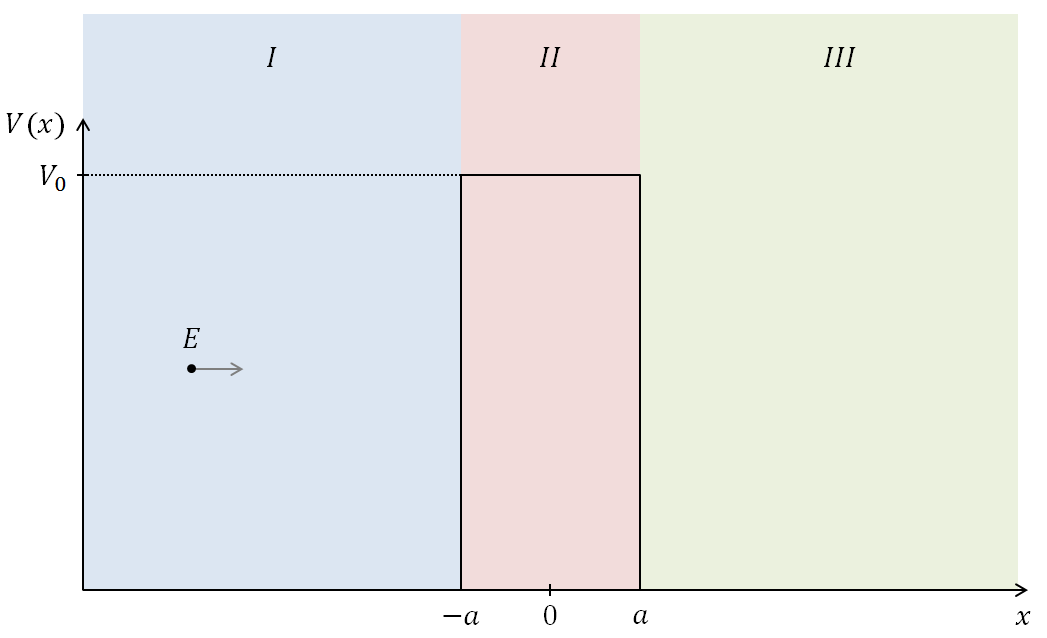
\includegraphics[width=0.7\textwidth]{tunneldiode/images/Kastenpotential.png}
\caption{Kastenpotential
\label{skript:Kastenpotential}}
\end{figure}

Die nachfolgenden Berechnungen sollen helfen, den Tunneleffekt zu verstehen.  Als erstes betrachten wir die statin"are Schr"odingergleichung f"ur die Wellenfunktion $\Phi(x)$. Dabei ist $m$ die Masse und $E$ die Energie des Teilchens.
\[
E\Phi(x) = -\frac{\hbar^2}{2m}\frac{d^2}{dx^2}\Phi(x) + V(x)\Phi(x)
\]
Im Bereich \RM{1} und \RM{3} verwenden wir f"ur die Wellenfunktion den allgemeine Ansatz
\[
\Phi(x) = Ae^{ikx}+Be^{-ikx}.
\]
F"ur $k$ gilt dabei
\[
k = \sqrt{\frac{2mE}{\hbar^2}}.
\]
Abgeleitet vom allgemeinen Ansatz m"ussen jetzt nur noch $A$ und $B$ bestimmt werden. Im Bereich \RM{1} ist
\[
A = 1 \text{ und } B = R
\]
da $A$ der Koeffizient der einlaufenden Welle ist und dieser Betragsm"assig als 1 angenommen wird. Diese Annahme ist notwendig, da sich die genaue Anzahl der Teilchen nicht ermitteln l"asst. $B$ ist der Koeffizient der auslaufende Welle. Das $R$ steht somit f"ur die Anzahl reflektierter Teilchen. Somit vereinfacht sich die Gleichung im Bereich \RM{1} zu
\[
\Phi_\RM{1}(x) = e^{ikx} + Re^{-ikx}.
\]

Im Bereich \RM{3} gilt
\[
A = T \text{ und } B = 0.
\]
Auch hier ist $A$ der Koeffizient der einlaufenden Welle und damit der transmittierten Teilchen, also $T$. Die m"oglicherweise in diesem Bereich reflektierten Teilchen interessieren uns nicht. Deshalb setzen wir $B$ auf 0. Somit erhalten wir f"ur den Bereich \RM{3} die Gleichung
\[
\Phi_\RM{3}(x) = Te^{ikx}.
\]
F"ur die Wellenfunktion im Bereich \RM{2} lautet die Gleichung
\[
\Phi_\RM{2}(x) = \alpha e^{\kappa x} + \beta e^{-\kappa x}
\]
da wir in der Potentialbarriere einen exponentiellen Abfall oder Anstieg erwarten. $\kappa$ ist
\[
\kappa = \sqrt{\frac{2m}{\hbar^2}(V_0 - E)}.
\]
Damit wir die vier Unbekannten $\alpha$, $\beta$, $R$ und $T$ bestimmen k"onnen, m"ussen wir Gemeinsamkeiten der Wellenfunktionen an den "Ubergangsstellen zwischen den Bereichen ausnutzen. Damit die Wellenfunktion ohne Spr"unge zusammengesetzt werden kann muss
\[
\Phi_\RM{1}(-a) = \Phi_\RM{2}(-a)
\]
\[
\Phi_\RM{2}(a) = \Phi_\RM{3}(a)
\]
\[
\Phi_\RM{1}'(-a) = \Phi_\RM{2}'(-a)
\]
\[
\Phi_\RM{2}'(a) = \Phi_\RM{3}'(a)
\]
gelten. Somit haben wir ein Gleichungssystem mit vier Gleichungen f"ur vier Unbekannte. Wir brauchen also die Ableitungen der Wellenfunktionen in den drei Bereichen.
\[
\Phi_\RM{1}'(x) = ike^{ikx} - Rike^{-ikx}
\]
\[
\Phi_\RM{2}'(x) = \alpha \kappa e^{\kappa x} - \beta \kappa e^{-\kappa x}
\]
\[
\Phi_\RM{3}'(x) = Tike^{ikx}
\]


%TODO: Überleitung zur Berechnung mit Matrizen
%      geometrischer Aufbau der Tunneldiode vs. Siliziumdiode
%	   Rückkehr zur Tunneldiode -> Wie der Tunneleffekt da auftritt
\section{"Ubergangsmatrix}
Die Matrix
\[
\begin{pmatrix}
\frac{i\,e^{2\,i\,a\,k}\,\left(\kappa-k\right)\,\left(\kappa+k
 \right)\,\sinh \left(2\,a\,\kappa\right)+2\,k\,e^{2\,i\,a\,k}\,
 \kappa\,\cosh \left(2\,a\,\kappa\right)}{2\,k\,\kappa}
&
\frac{i\,
 \left(\kappa^2+k^2\right)\,\sinh \left(2\,a\,\kappa\right)}{2\,
 k\,\kappa}
\\
-\frac{i\,\left(\kappa^2+k^2\right)\,\sinh \left(2\,a\,
 \kappa\right)}{2\,k\,\kappa}
&
\frac{2\,k\,e^ {- 2\,i\,a\,k }\,
 \kappa\,\cosh \left(2\,a\,\kappa\right)-i\,e^ {- 2\,i\,a\,k }\,
 \left(\kappa-k\right)\,\left(\kappa+k\right)\,\sinh \left(2\,a\,
 \kappa\right)}{2\,k\,\kappa}
\end{pmatrix}
\]
berechnet die Amplitude der einfallenden und reflektierten Wellen
aus den Amplituden der Wellen rechts von der Barriere.
Davon brauchen wir nur die erste Spalte.

In allen Termen kann man $2a$ durch die Dicke $l$ der Barriere ersetzen.
Die erste Spalte gibt wieder, wieviel mal wahrscheinlicher ein einfallendes
teilchen im Vergleich zu einem durchgelassenen Teilchen ist:
\[
\begin{pmatrix}
\displaystyle
e^{ilk}\biggl(\cosh(l\kappa)
+\frac{i}{2}\biggl(\frac{\kappa}{k}-\frac{k}{\kappa}\biggr)\sinh(l\kappa)
\biggr)
\\
\displaystyle
- \frac{i}{2}
\biggl(\frac{\kappa}{k}+\frac{k}{\kappa}\biggr)
\sinh(l\kappa)
\end{pmatrix}
\]

\section{Amplitude der Wellen links von der Barriere}
Die Amplitude der einfallenden Welle ist
\begin{align*}
A_{\text{in}}
&=
\frac{i e^{i l k} (\kappa-k) (\kappa+k) 
 \sinh (l \kappa)+2 k e^{i l k} \kappa \cosh 
 (l \kappa)}{2 k \kappa}
\\
&=
e^{i l k}
\biggl(
\frac{
i
(\kappa^2-k^2)
}{2 k \kappa}
\sinh (l \kappa)
+
\cosh (l \kappa)
\biggr)
\\
|A_{\text{in}}|^2
&=
\cosh^2(l\kappa)
+
\frac14\biggl(
\frac{\kappa}{k}-\frac{k}{\kappa}
\biggr)^2
\sinh^2(l\kappa)
\\
A_{\text{reflect}}
&=
-\frac{i}{2}
\biggl(\frac{\kappa}{k}+\frac{k}{\kappa}\biggr)
\sinh (2 a \kappa)
\\
|A_{\text{reflect}}|^2
&=
\frac14
\biggl(\frac{\kappa}{k}+\frac{k}{\kappa}\biggr)^2
\sinh^2 (2 a \kappa)
\end{align*}

\section{Wellenfunktion in der Barriere}
Betragsquadrat der Wellenfunktion in der Barriere
\begin{align*}
|\psi_{\text{Barrier}}(x)|^2
&=
\frac{
(\kappa^2+k^2)\cosh (2\kappa x-2a\kappa)+(\kappa-k)(\kappa+k)
}{
2\kappa ^2
}
\\
&=
\frac12
\biggl(1+\frac{k^2}{\kappa^2}\biggr)
\cosh (2\kappa(x-a))
+
\frac12
\biggl(1-\frac{k^2}{\kappa^2}\biggr)
\\
&=
\cosh (2\kappa(x-a))+1
+
\frac{k^2}{\kappa^2}
(\underbrace{\cosh (2\kappa(x-a))-1}_{\ge 0})
>0
\end{align*}
f"ur $x\le a$.

Intensit"atsverh"altnis zwischen einfallender und durchgelassener
Welle
\[
\frac{1}{
\displaystyle
\cosh^2 l\kappa 
+
4\biggl(\displaystyle\frac{\kappa}{k}-\frac{k}{\kappa}\biggr)^2\sinh^2l\kappa
}
\]

Intensit"atsverh"altnis zwischen einfallender und reflektierter
Welle:
\[
\frac{
4\coth^2l\kappa + \biggl(\displaystyle\frac{\kappa}{k}-\frac{k}{\kappa}\biggr)^2
}{
\biggl(\displaystyle\frac{\kappa}{k}+\frac{k}{\kappa}\biggr)^2
}
\]

F"ur die Amplitude der Wellenfunktion links von der Barriere
ist es n"utzlich, die beiden Gr"ossen
\begin{align*}
K_p&=\frac{\kappa^2+k^2}{2\kappa k}
\\
K_m&=\frac{\kappa^2-k^2}{2\kappa k}
\end{align*}
als Abk"urzung zu verwenden. Damit kann man die von \texttt{maxima} berechnete
Wahrscheinlichkeit wie folgt umformen:
\begin{align*}
|\psi_{\text{left}}(x)|^2
&=
\frac{
-
2 \sin (2 \delta) k \kappa (\kappa^2+k^2) \sinh (4 a \kappa)
+
(\kappa^2+k^2)^2 \cosh (4 a \kappa)
}{4 k ^2 \kappa^2}
\\
&\qquad
+
\frac{
-
\cos (2 \delta) (\kappa-k) (\kappa+k) (\kappa^2+k^2) \cosh (4 a \kappa)
-
(\kappa-k)^2 (\kappa+k)^2
}{4 k ^2 \kappa^2}
\\
&\qquad
+
\frac{
\cos (2 \delta) (\kappa-k) (\kappa+k) (\kappa^2+k^2)
}{4 k ^2 \kappa^2}
\\
&=
-
\frac{
2 \sin (2 \delta) k \kappa (\kappa^2+k^2) \sinh (4 a \kappa)
}{4 k ^2 \kappa^2}
+
\frac{
(\kappa^2+k^2)^2 \cosh (4 a \kappa)
}{4 k ^2 \kappa^2}
\\
&\qquad
-
\frac{
\cos (2 \delta) (\kappa-k) (\kappa+k) (\kappa^2+k^2) \cosh (4 a \kappa)
}{4 k ^2 \kappa^2}
-
\frac{
(\kappa-k)^2 (\kappa+k)^2
}{4 k ^2 \kappa^2}
\\
&\qquad
+
\frac{
\cos (2 \delta) (\kappa-k) (\kappa+k) (\kappa^2+k^2)
}{4 k ^2 \kappa^2}
\\
&=
-
\frac{
(\kappa^2+k^2)
}{2 k \kappa}
\sin (2 \delta)
\sinh (4 a \kappa)
+
\frac{
(\kappa^2+k^2)^2
}{4 k ^2 \kappa^2}
\cosh (4 a \kappa)
\\
&\qquad
-
\frac{
(\kappa^2-k^2) (\kappa^2+k^2)
}{4 k ^2 \kappa^2}
\cos (2 \delta)
\cosh (4 a \kappa)
-
\frac{
(\kappa-k)^2 (\kappa+k)^2
}{4 k ^2 \kappa^2}
\\
&\qquad
+
\frac{
(\kappa^2-k^2) (\kappa^2+k^2)
}{4 k ^2 \kappa^2}
\cos (2 \delta)
\\
&=
-
K_p
\sin (2 \delta)
\sinh (4 a \kappa)
+
K_p^2
\cosh (4 a \kappa)
-
K_pK_m
\cos (2 \delta)
\cosh (4 a \kappa)
-
K_m^2
+
K_pK_m
\cos (2 \delta)
\\
&=
-
K_p \sin (2 \delta) \sinh (4 a \kappa)
+
K_p^2 \cosh (4 a \kappa)
-
K_pK_m \cos (2 \delta) (\cosh (4 a \kappa)-1)
-
K_m^2
\end{align*}


\section{Fall $E>V_0$}

\[
\begin{pmatrix}
\frac{2\,k\,e^{2\,i\,a\,k}\,\kappa\,\cos \left(2\,a\,\kappa
 \right)-i\,e^{2\,i\,a\,k}\,\left(i\,\kappa^2+\kappa^2-i\,k^2+k^2
 \right)\,\sin \left(2\,a\,\kappa\right)}{2\,k\,\kappa}
&
-\frac{i\,
 \left(\kappa+k\right)\,\left(i\,\kappa+\kappa+i\,k-k\right)\,\sin 
 \left(2\,a\,\kappa\right)}{2\,k\,\kappa}
\\
\frac{i\,\left(\kappa-
 k\right)\,\left(i\,\kappa+\kappa-i\,k+k\right)\,\sin \left(2\,a\,
 \kappa\right)}{2\,k\,\kappa}
&
\frac{i\,e^ {- 2\,i\,a\,k }\,\left(i
 \,\kappa^2+\kappa^2-i\,k^2+k^2\right)\,\sin \left(2\,a\,\kappa
 \right)+2\,k\,e^ {- 2\,i\,a\,k }\,\kappa\,\cos \left(2\,a\,\kappa
 \right)}{2\,k\,\kappa}
\end{pmatrix}
\]


%
% Tunneldioden-Oszillator
%
% (c) 2015 Prof Dr Andreas Mueller, Hochschule Rapperswil
%
\section{Tunneldioden-Oszillator}
\rhead{Tunneldioden-Oszillator}
\begin{figure}
\centering
\includestandalone{tunneldiode/schematic}
\caption{Oszillator-Schaltung mit Tunneldiode
\label{tunnel:tunneldioden-oszillator}}
\end{figure}
Eine Tunneldiode kann dazu verwendet werden, einen Schwingkreis zu
entd"ampfen und so einen einfachen Oszillator zu konstruieren.
Eine m"ogliche Schaltung zeigt Abbildung~\ref{tunnel:tunneldioden-oszillator}.

Um die Schaltung zu analysieren, brauchen wir ein Modell f"ur die
Charakteristik der Tunneldiode. Wir nehmen dazu an, dass $U_0$ kleiner
ist also die Spannung, bei der die normale Diodenleitung einsetzt.
Dann k"onnen wir zwischen dem Strom $I_T$ durch die Tunneldiode
und der Vorw"artsspannung $U_T$ einen linearen Zusammenhang
\begin{equation}
I_T=b-aU_T
\label{tunnel:charakteristik}
\end{equation}
annehmen. $b$ entspricht in etwa dem Peak-Strom $I_{\text{peak}}$, der
Tunnelstrom bricht bei der Spannung $b/a$ zusammen.

Jetzt k"onnen wir die Differentialgleichung f"ur die Spannung $U(t)$
aufstellen. Wir bezeichnen den Spannungsabfall "uber dem Bauteil $X$
mit $U_X$ und den Strom durch das Bauteil mit $I_X$. Die Knotengleichung
bei $U(t)$ besagt:
\[
I_L+I_C=I_T
\]
Daraus und aus $U_T=U_0-U(t)$ kann $I_T$ mit Hilfe der angenommenen
Charakteristik~(\ref{tunnel:charakteristik}) der Tunneldiode eliminert werden.
Es ist
\begin{equation}
I_L+I_C=b-aU_T=b-a(U_0-U(t)).
\label{tunnel:knotengleichung}
\end{equation}
F"ur die Str"ome im Schwingkreis gilt
\begin{align*}
C\dot U_C&=I_C \qquad\text{und}\\
U_L&=L\dot I_L
\end{align*}
Nat"urlich ist $U_L=U_C=U(t)$.
Da wir in der zweiten Gleichung nur die Ableitung von $I_L$ nach
der Zeit haben, leiten wir
auch die erste und die Gleichung~(\ref{tunnel:knotengleichung}) nach
der Zeit ab, und setzen die abgeleiteten Str"ome
in~(\ref{tunnel:knotengleichung}) ein.
So erhalten wir die Differentialgleichung
\begin{equation*}
\frac1{L}U(t) +C\ddot U(t)=a\dot U(t)
\end{equation*}
oder
\begin{equation}
\ddot U(t)
-\frac{a}{C}\dot U(t)
+\frac1{LC}U(t)
=0.
\label{tunnel:dgl1}
\end{equation}
F"ur $a=0$ wird daraus eine gew"ohnliche Schwingungsdifferentialgleichung
mit Kreisfrequenz $\omega_0^2=1/LC$.

\begin{figure}
\centering
\includegraphics{tunneldiode/tunnel-8.pdf}
\caption{Designparameter $L$ und $C$ des Tunneldioden-Oszillators nach
Abbildung~\ref{tunnel:tunneldioden-oszillator}. 
Die Hyperbeln verbinden Punkte gleicher Eigenfrequenz des Schwingkreises.
Dass hellgraue Gebiet wird ausgeschlossen durch die Bedingung, dass die
Kapazit"at gross genug sein muss.
Das dunkelgraue Gebiet schliesst Werte der Induktivit"at aus, wenn die
Kreisfrequenz $\omega$ erreicht werden soll.
\label{tunnel:designparameter}}
\end{figure}

Das charakteristische Polynom der Differentialgleichung~(\ref{tunnel:dgl1})
ist
\[
\lambda^2-\frac{a}{C}\lambda +\omega_0^2\lambda=0
\]
mit den Nullstellen
\[
\lambda_\pm = \frac{a}{2C}\pm\sqrt{\frac{a^2}{4C^2}-\omega_0^2}.
\]
Damit tats"achlich Schwingungsl"osungen entstehen, muss der Radikand
negativ sein, es muss also gelten
\[
\frac{a^2}{4C^2}<\frac1{LC}
\qquad\Rightarrow\qquad
\frac{C}{L} > \frac{a^2}{4}.
\]
Die Kapazit"at $C$ muss also ausreichend gross sein.
Abbildung~\ref{tunnel:designparameter} zeigt den Raum der Design-Parameter
$C$ und $L$.

Eine grosse Kapazit"at $C$ bewirkt aber auch, dass der Koeffizient
$-a/C$ des $\dot U(t)$-Terms kleiner wird. Mit zunehmender Kapazit"at
wird als die Entd"ampfung geringer, und je nach parasit"arer D"ampfung
kann es schwierig werden, dass die Schaltung "uberhaupt anschwingt.

Die Schwingungsfrequenz wird f"ur $a\ne 0$ modifiziert zu
\begin{equation}
\omega
=
\sqrt{
\frac{1}{LC}
-
\frac{a^2}{4C^2}
}.
\label{tunnel:oszillatorfrequenz}
\end{equation}
Bei vorgegebener Schwingungsfrequenz und Induktivit"at ist dies eine
quadratische Gleichung f"ur $C$, wir schreiben sie in der gebr"auchlicheren
Form
\[
\omega^2 C^2 -\frac1{L}C+\frac{a^2}{4}=0.
\]
Diese Gleichung hat nur dann reelle L"osungen f"ur $C$, wenn die Diskriminante
positiv ist, also
\begin{equation}
\begin{aligned}
\frac1{L^2}-4\omega^2\frac{a^2}4&>0
&
&\Rightarrow&
\frac1{L^2}&>\omega^2a^2
&
&\Rightarrow&
L<&\frac1{a\omega}
\end{aligned}
\end{equation}
Wenn also die Kreisfrequenz $\omega$ angestrebt werden soll, dann darf die
Induktivit"at nicht zu gross sein.
Dies wird in Abbildung~\ref{tunnel:designparameter} durch das dunkelgraue
Gebiet dargestellt.

\begin{beispiel}
Die in diesem Kapitel genauer untersuchte Tunneldiode 1N3721 hat einen
Spitzenstrom von $I_{\text{peak}}=25\,\text{mA}$, der Tunnelstrom
bricht bei $450\,\text{mV}$ zusammen.
Wir k"onnen also von $a=25/450=0.0555\text{A/V}$ ausgehen.
Mit einer Induktivit"at von $L=0.1\mu\text{H}$ l"asst sich dann bestenfalls
die Kreisfrequenz
$\omega=1/(aL)=1/(10^{-7}\cdot 0.055)=180\cdot 10^6\,\text{s}^{-1}$
erreichen,
also die Frequenz $28.7\,\text{MHz}$.
Die Kapazit"at muss mindestens $C>La^2/4=77\text{pF}$ sein.

Mit einem $100\,\text{nF}$-Kondensator gilt f"ur die Eigenkreisfrequenz
$\omega_0$ des Schwingkreises $\omega_0^2=1/LC=10^{14}$, die Eigenfrequenz
ist also etwa $1.5915\,\text{MHz}$.
F"ur die Frequenz des Oszillators muss allerdings die
Formel~(\ref{tunnel:oszillatorfrequenz}) verwendet werden.
Da aber in unserem Fall $a^2/4\simeq 0.00077$ ziemlich klein ist, ist
die Frequenz fast gleich wie die Eigenfrequenz des Schwingkreises.
Anwendung der Formel~(\ref{tunnel:oszillatorfrequenz})
ergibt $1.5909\,\text{MHz}$, also tats"achlich nur ein sehr kleiner
Unterschied zur Eigenfrequenz.
\end{beispiel}



\printbibliography[heading=subbibliography]
\end{refsection}

